\documentclass[tikz,border=6pt]{standalone}
\usepackage{tikz}
\begin{document}
\small
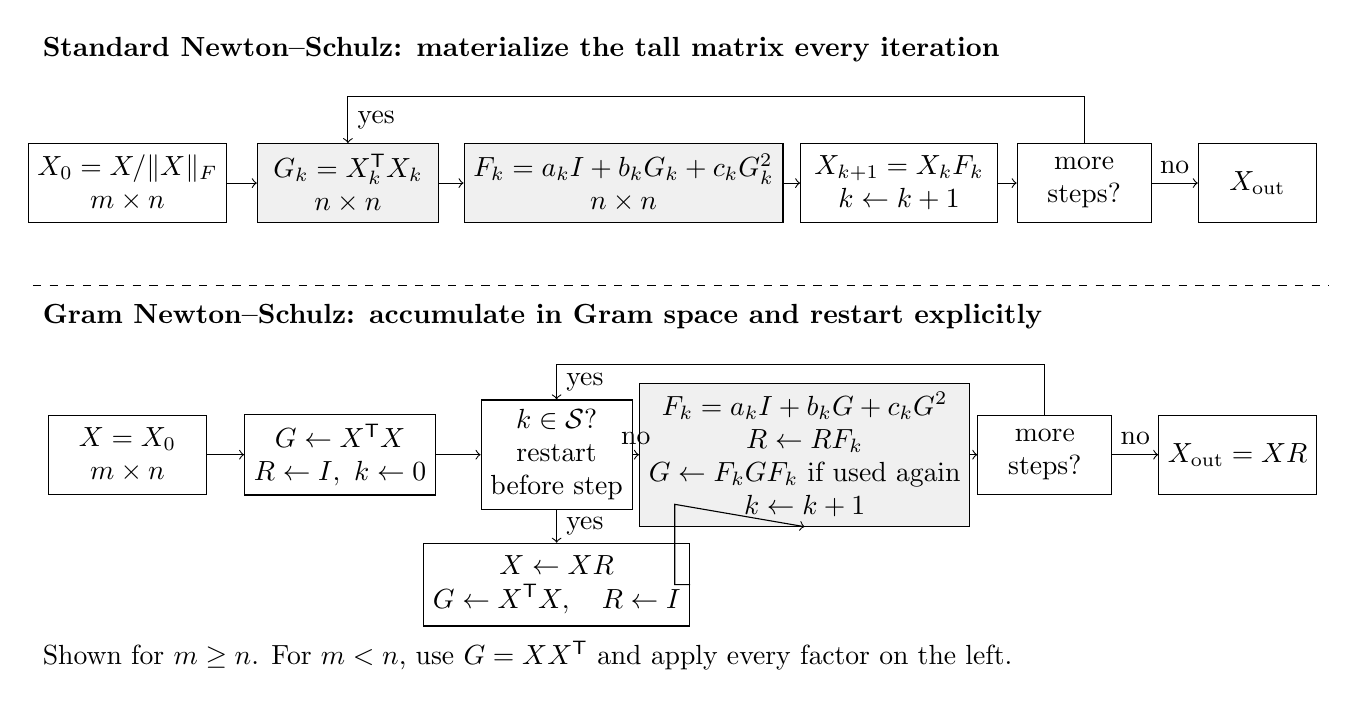
\begin{tikzpicture}
  \node[anchor=west,font=\bfseries] at (-1.0,5.35)
    {Standard Newton--Schulz: materialize the tall matrix every iteration};

  \node[draw,minimum width=2.0cm,minimum height=1.0cm,align=center] (stdinput) at (0.2,3.65)
    {$X_0=X/\|X\|_F$\\$m\times n$};
  \node[draw,minimum width=2.3cm,minimum height=1.0cm,align=center,fill=gray!12] (stdgram) at (3.0,3.65)
    {$G_k=X_k^{\mathsf T}X_k$\\$n\times n$};
  \node[draw,minimum width=3.3cm,minimum height=1.0cm,align=center,fill=gray!12] (stdfactor) at (6.5,3.65)
    {$F_k=a_kI+b_kG_k+c_kG_k^2$\\$n\times n$};
  \node[draw,minimum width=2.5cm,minimum height=1.0cm,align=center] (stdupdate) at (10.0,3.65)
    {$X_{k+1}=X_kF_k$\\$k\leftarrow k+1$};
  \node[draw,minimum width=1.7cm,minimum height=1.0cm,align=center] (stdmore) at (12.35,3.65)
    {more\\steps?};
  \node[draw,minimum width=1.5cm,minimum height=1.0cm,align=center] (stdout) at (14.55,3.65)
    {$X_{\rm out}$};

  \draw[->] (stdinput.east) -- (stdgram.west);
  \draw[->] (stdgram.east) -- (stdfactor.west);
  \draw[->] (stdfactor.east) -- (stdupdate.west);
  \draw[->] (stdupdate.east) -- (stdmore.west);
  \draw[->] (stdmore.east) -- node[above] {no} (stdout.west);
  \draw[->] (stdmore.north) -- (12.35,4.75) -- (3.0,4.75) -- node[right] {yes} (stdgram.north);

  \draw[dashed] (-1.0,2.35) -- (15.45,2.35);

  \node[anchor=west,font=\bfseries] at (-1.0,1.95)
    {Gram Newton--Schulz: accumulate in Gram space and restart explicitly};

  \node[draw,minimum width=2.0cm,minimum height=1.0cm,align=center] (gnsinput) at (0.2,0.2)
    {$X=X_0$\\$m\times n$};
  \node[draw,minimum width=2.4cm,minimum height=1.0cm,align=center] (gnsinit) at (2.9,0.2)
    {$G\leftarrow X^{\mathsf T}X$\\$R\leftarrow I,\ k\leftarrow0$};
  \node[draw,minimum width=1.9cm,minimum height=1.25cm,align=center] (resetquery) at (5.65,0.2)
    {$k\in\mathcal S$?\\restart\\before step};
  \node[draw,minimum width=3.9cm,minimum height=1.55cm,align=center,fill=gray!12] (gnsupdate) at (8.8,0.2)
    {$F_k=a_kI+b_kG+c_kG^2$\\$R\leftarrow RF_k$\\$G\leftarrow F_kGF_k$ if used again\\$k\leftarrow k+1$};
  \node[draw,minimum width=1.7cm,minimum height=1.0cm,align=center] (gnsmore) at (11.85,0.2)
    {more\\steps?};
  \node[draw,minimum width=2.0cm,minimum height=1.0cm,align=center] (gnsout) at (14.3,0.2)
    {$X_{\rm out}=XR$};
  \node[draw,minimum width=3.3cm,minimum height=1.05cm,align=center] (restart) at (5.65,-1.45)
    {$X\leftarrow XR$\\$G\leftarrow X^{\mathsf T}X,\quad R\leftarrow I$};

  \draw[->] (gnsinput.east) -- (gnsinit.west);
  \draw[->] (gnsinit.east) -- (resetquery.west);
  \draw[->] (resetquery.east) -- node[above] {no} (gnsupdate.west);
  \draw[->] (resetquery.south) -- node[right] {yes} (restart.north);
  \draw[->] (restart.east) -- (7.15,-1.45) -- (7.15,-0.43) -- (gnsupdate.south);
  \draw[->] (gnsupdate.east) -- (gnsmore.west);
  \draw[->] (gnsmore.east) -- node[above] {no} (gnsout.west);
  \draw[->] (gnsmore.north) -- (11.85,1.35) -- (5.65,1.35) -- node[right] {yes} (resetquery.north);

  \node[anchor=west,align=left] at (-1.0,-2.35)
    {Shown for $m\ge n$.  For $m<n$, use $G=XX^{\mathsf T}$ and apply every factor on the left.};
\end{tikzpicture}
\end{document}
